\documentclass{article}
\usepackage{ifthen}
\usepackage{amssymb}
\usepackage{multicol}
\usepackage{graphicx}
\usepackage[absolute]{textpos}
\usepackage{amsmath, amscd, amssymb, amsthm, latexsym}
\usepackage{xspace,rotating,dsfont,ifthen}
\usepackage[spanish,activeacute]{babel}
\usepackage[utf8]{inputenc}
\usepackage{pgfpages}
\usepackage{pgf,pgfarrows,pgfnodes,pgfautomata,pgfheaps,xspace,dsfont}
\usepackage{listings}
\usepackage{multicol}
\usepackage{todonotes}
\usepackage{url}
\usepackage{float}
\usepackage{framed,mdframed}
\usepackage{cancel}

\usepackage[strict]{changepage}


\makeatletter


\newcommand\hfrac[2]{\genfrac{}{}{0pt}{}{#1}{#2}} %\hfrac{}{} es un \frac sin la linea del medio

\newcommand\Wider[2][3em]{% \Wider[3em]{} reduce los m\'argenes
\makebox[\linewidth][c]{%
  \begin{minipage}{\dimexpr\textwidth+#1\relax}
  \raggedright#2
  \end{minipage}%
  }%
}


\@ifclassloaded{beamer}{%
  \newcommand{\tocarEspacios}{%
    \addtolength{\leftskip}{4em}%
    \addtolength{\parindent}{-3em}%
  }%
}
{%
  \usepackage[top=1cm,bottom=2cm,left=1cm,right=1cm]{geometry}%
  \usepackage{color}%
  \newcommand{\tocarEspacios}{%
    \addtolength{\leftskip}{3em}%
    \setlength{\parindent}{0em}%
  }%
}

\usepackage{caratula}
\usepackage{enumerate}
\usepackage{hyperref}
\usepackage{graphicx}
\usepackage{amsfonts}
\usepackage{enumitem}
\usepackage{amsmath}

\decimalpoint
\hypersetup{colorlinks=true, linkcolor=black, urlcolor=blue}
\setlength{\parindent}{0em}
\setlength{\parskip}{0.5em}
\setcounter{tocdepth}{2} % profundidad de indice
\setcounter{section}{5} % nro de section
\renewcommand{\thesubsubsection}{\thesubsection.\Alph{subsubsection}}
\graphicspath{ {images/} }

% End latex config

\begin{document}

\titulo{Práctica 6}
\fecha{2do cuatrimestre 2021}
\materia{Álgebra I}
\integrante{Yago Pajariño}{546/21}{ypajarino@dc.uba.ar}

%Carátula
\maketitle
\newpage

%Indice
\tableofcontents
\newpage

% Aca empieza lo propio del documento
\section{Práctica 6}

\subsection{Ejercicio 1}

\subsubsection{Pregunta i}

Paso a polares:
\begin{itemize}
    \item $ 5i = 5(\cos(\frac{\pi}{2}) + i\sin(\frac{\pi}{2})) $
    \item $ (1+i)^4 = (\sqrt{2})^4 .(\cos(\pi)+i\sin(\pi)) $
\end{itemize}

Luego,
\begin{align*}
    z &= 4.5(\cos(\pi + \frac{\pi}{2})+i\sin(\pi +\frac{\pi}{2})) \\
    &= 20(\cos(\frac{3\pi}{2})+i\sin(\frac{3\pi}{2})) \\
\end{align*}

Así,
\begin{itemize}
    \item $ Re(z) = 20. \cos(\frac{3\pi}{2}) = 0 $
    \item $ Im(z) = 20. \sin(\frac{3\pi}{2}) = -20 $
    \item $ |z| = 20 $
    \item $ Re(z^{-1}) = 0 $
    \item $ iz = 20(\cos(2\pi)+i\sin(2\pi)) \implies Im(iz) = 0 $
\end{itemize}

\subsubsection{Pregunta ii}

\begin{align*}
    z &= (\sqrt[]{2} + \sqrt[]{3}i)^2.(\overline{1-3i}) \\
    &= (2 + 2\cdot \sqrt[]{2} \cdot\sqrt[]{3}i - 3).(1 + 3i) \\
    &= (-1 + 2\cdot \sqrt[]{6}i).(1 + 3i) \\
    &= -1 - 3i + 2 \cdot\sqrt[]{6}i - 6 \cdot \sqrt[]{6} \\
    &= -1 - 6 \cdot \sqrt[]{6} + (2 \cdot\sqrt[]{6} - 3)i \\
\end{align*}

\begin{itemize}
    \item $ Re(z) = -1 - 6 \cdot \sqrt[]{6} $
    \item $ Im(z) = 2 \cdot\sqrt[]{6} - 3 $
    \item $ |z| = \sqrt{(-1 - 6 \cdot \sqrt[]{6})^2 + (2 \cdot\sqrt[]{6} - 3)^2} = \sqrt[]{250} = 5\cdot\sqrt[]{10} $
\end{itemize}

\subsubsection{Pregunta iii}

Paso a polares,

$ i^{17} = \cos(17.\frac{\pi}{2}) + i\sin(17\frac{\pi}{2}) $

$ \frac{1}{2} = \frac{1}{2}.(\cos(0) + i\sin(0)) $

$ i = \cos(\frac{\pi}{2}) +i\sin(\frac{\pi}{2}) $

$ (1-i)^3 = (\sqrt[]{2})^3(\cos(3.\frac{7}{4}\pi)+i\sin(3.\frac{7}{4}\pi)) $

Luego,
\begin{align*}
    \frac{1}{2} . i . (1+i)^3 &= \frac{1}{2}.(\sqrt[]{2})^3.\left(\cos(\frac{\pi}{2} + \frac{21}{4}\pi) +i\sin(\frac{\pi}{2} + \frac{21}{4}\pi)\right) \\
    &= \frac{\sqrt[]{2}^3}{2}.\left(\cos\left(\frac{23}{4}\pi\right) +i\sin\left(\frac{23}{4}\pi\right)\right) \\
\end{align*}
Entonces,
\begin{align*}
    z &= \frac{\sqrt[]{2}^3}{2}.\left(\cos\left((\frac{17}{2} + \frac{23}{4})\pi\right) +i\sin\left((\frac{17}{2} + \frac{23}{4})\pi\right)\right) \\
    &= \frac{\sqrt[]{2}^3}{2}.\left(\cos\left(\frac{57}{4}\pi\right) +i\sin\left(\frac{57}{4}\pi\right)\right) \\
\end{align*}

\begin{itemize}
    \item $ Re(z) = \frac{\sqrt[]{2}^3}{2} . \cos\left(\frac{57}{4}\pi\right) $
    \item $ Im(z) = \frac{\sqrt[]{2}^3}{2} . \sin\left(\frac{57}{4}\pi\right) $
    \item $ |z| = \frac{\sqrt[]{2}^3}{2} $
    \item $ Re(z^{-1}) = \cos\left(\frac{57}{4}\pi\right) $
    \item $ Im(iz) = \frac{\sqrt[]{2}^3}{2} . \sin\left(\frac{59}{4}\pi\right) $
\end{itemize}

\subsubsection{Pregunta iv}
TODO

\subsubsection{Pregunta v}
TODO

\subsection{Ejercicio 2}

\begin{enumerate}
    \item 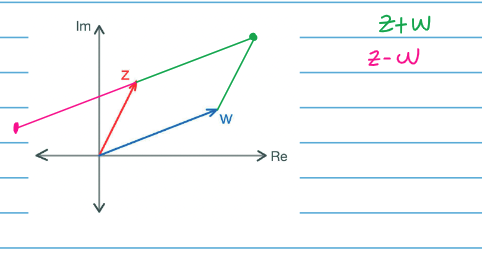
\includegraphics[width=250px]{6.2.1}
    \item 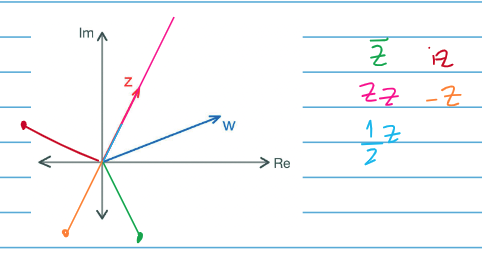
\includegraphics[width=250px]{6.2.2}
    \item 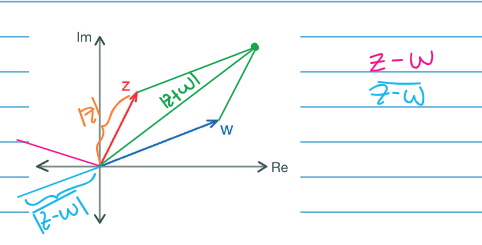
\includegraphics[width=250px]{6.2.3}
\end{enumerate}


\end{document}
